\documentclass[12pt,a4paper]{article}

\usepackage[utf8]{inputenc}
\usepackage[T1]{fontenc}
\usepackage[brazilian]{babel}
\usepackage{amsmath}
\usepackage{graphicx}
\usepackage{geometry}
\usepackage{float}
\usepackage{hyperref}
\usepackage{booktabs,tabularx,threeparttable,caption}

\geometry{top=2.5cm, bottom=2.5cm, left=3cm, right=3cm}

\title{Atividade 4: Redes Convolucionais (CNN) \\ \large Disciplina: Redes Neurais Artificiais}
\author{Programa de Pós-Graduação em Ciência da Computação (PPGCC-UNESP)}
\date{\today}

\begin{document}

\maketitle

\section{Introdução e Implementação}

Este documento apresenta os resultados da implementação e avaliação de redes neurais convolucionais (CNNs) para classificação de imagens no conjunto de dados CIFAR-10. O dataset contém imagens RGB de 32$\times$32 pixels distribuídas em 10 classes: avião, carro, pássaro, gato, cervo, cachorro, sapo, cavalo, navio e caminhão.

A CNN foi construída do zero utilizando o módulo \texttt{nn.Module} do PyTorch, sem o uso de modelos prontos. A arquitetura é parametrizável, permitindo instanciar diferentes topologias variando o número de camadas convolucionais, número de filtros e taxa de dropout. Cada bloco convolucional é composto por uma camada \texttt{Conv2d}, ativação \texttt{ReLU} e \texttt{MaxPool2d} (kernel $2\times2$, stride 2). Após o extrator de características, a cabeça classificadora consiste em três camadas totalmente conectadas (\texttt{FC1} e \texttt{FC2} com 200 neurônios cada, \texttt{FC3} com 10 saídas), com \texttt{Dropout} entre elas. A função de perda utilizada é a \texttt{CrossEntropyLoss} e os otimizadores avaliados são SGD e Adam.

O conjunto de treino (50.000 imagens) foi dividido em 90\% para treino efetivo e 10\% para validação, com \textit{early stopping} de paciência 5 épocas. O conjunto de teste (10.000 imagens) foi utilizado exclusivamente para avaliação final. As imagens foram normalizadas para média 0,5 e desvio padrão 0,5 por canal.

\section{Arquiteturas e Experimentos}

Foram testadas 36 arquiteturas combinando os seguintes hiperparâmetros:

\begin{itemize}
    \item \textbf{Otimizadores:} SGD, Adam
    \item \textbf{Camadas convolucionais:} 2, 3, 4
    \item \textbf{Filtros:} 32, 64, 128
    \item \textbf{Dropout nas camadas FC:} $p = 0{,}1$ e $p = 0{,}3$
\end{itemize}

Todos os modelos foram treinados por até 30 épocas com \textit{early stopping}. A seguir, apresentam-se os resultados completos no conjunto de teste.

\begin{table}[H]
\centering
\caption{Resultados completos no conjunto de teste -- CIFAR-10}
\label{tab:full_results}
\scriptsize
\setlength{\tabcolsep}{4pt}
\begin{tabular}{lllllll}
\toprule
\textbf{Otim.} & \textbf{Conv} & \textbf{Filtros} & \textbf{Dropout} & \textbf{Test Loss} & \textbf{Test Acc} & \textbf{Épocas} \\
\midrule
SGD & 2 & 32  & 0.1 & 1.5717 & 0.4305 & 30 \\
SGD & 2 & 32  & 0.3 & 1.6879 & 0.3900 & 30 \\
SGD & 2 & 64  & 0.1 & 1.4878 & 0.4575 & 30 \\
SGD & 2 & 64  & 0.3 & 1.5302 & 0.4490 & 30 \\
SGD & 2 & 128 & 0.1 & 1.3779 & 0.5005 & 30 \\
SGD & 2 & 128 & 0.3 & 1.4445 & 0.4789 & 30 \\
SGD & 3 & 32  & 0.1 & 1.9177 & 0.3056 & 30 \\
SGD & 3 & 32  & 0.3 & 2.2710 & 0.2494 & 30 \\
SGD & 3 & 64  & 0.1 & 1.8110 & 0.3452 & 30 \\
SGD & 3 & 64  & 0.3 & 1.8894 & 0.3090 & 30 \\
SGD & 3 & 128 & 0.1 & 1.6567 & 0.4000 & 30 \\
SGD & 3 & 128 & 0.3 & 1.7831 & 0.3477 & 30 \\
SGD & 4 & 32  & 0.1 & 2.3016 & 0.1023 & 30 \\
SGD & 4 & 32  & 0.3 & 2.2866 & 0.1347 & 30 \\
SGD & 4 & 64  & 0.1 & 2.2829 & 0.1352 & 30 \\
SGD & 4 & 64  & 0.3 & 2.2942 & 0.1996 & 30 \\
SGD & 4 & 128 & 0.1 & 2.2753 & 0.1693 & 30 \\
SGD & 4 & 128 & 0.3 & 2.2720 & 0.2148 & 30 \\
\midrule
Adam & 2 & 32  & 0.1 & 1.0548 & 0.7083 & 10 \\
Adam & 2 & 32  & 0.3 & 0.9303 & 0.7050 & 13 \\
Adam & 2 & 64  & 0.1 & 1.0858 & 0.7199 & 10 \\
Adam & 2 & 64  & 0.3 & 0.9838 & 0.7204 & 13 \\
Adam & 2 & 128 & 0.1 & 1.1261 & 0.7331 & 10 \\
Adam & 2 & 128 & 0.3 & 0.9431 & 0.7269 & 10 \\
Adam & 3 & 32  & 0.1 & 0.8228 & 0.7337 & 12 \\
Adam & 3 & 32  & 0.3 & 0.8069 & 0.7304 & 14 \\
Adam & 3 & 64  & 0.1 & 1.0178 & 0.7324 & 15 \\
Adam & 3 & 64  & 0.3 & 0.8406 & 0.7511 & 16 \\
Adam & 3 & 128 & 0.1 & 0.8726 & 0.7629 & 10 \\
Adam & 3 & 128 & 0.3 & \textbf{0.7672} & 0.7595 & 11 \\
Adam & 4 & 32  & 0.1 & 0.8440 & 0.7186 & 13 \\
Adam & 4 & 32  & 0.3 & 0.8374 & 0.7265 & 17 \\
Adam & 4 & 64  & 0.1 & 0.9404 & 0.7354 & 14 \\
Adam & 4 & 64  & 0.3 & 0.8777 & 0.7394 & 15 \\
Adam & 4 & 128 & 0.1 & 0.8780 & \textbf{0.7646} & 12 \\
Adam & 4 & 128 & 0.3 & 0.8770 & 0.7504 & 11 \\
\bottomrule
\end{tabular}
\begin{tablenotes}
  \footnotesize
  \item Valores em \textbf{negrito} indicam o melhor resultado em cada métrica.
\end{tablenotes}
\end{table}

\section{Análises e Discussão}

\subsection{Impacto do Otimizador}

A diferença mais marcante observada nos experimentos é a superioridade absoluta do Adam sobre o SGD no contexto de CNNs treinadas no CIFAR-10. Enquanto o Adam produziu acurácias entre 70\% e 76\%, todas as configurações com SGD ficaram abaixo de 51\%, e as arquiteturas com 4 camadas convolucionais e SGD chegaram a colapsar próximas à acurácia aleatória ($\approx$10\%), indicando falha de convergência. Esse comportamento contrasta com a atividade anterior (MLP), onde SGD e Adam apresentaram resultados mais equilibrados no dataset multiclasse. A taxa de aprendizado adaptativa do Adam mostra-se essencial para navegar a superfície de perda mais complexa de uma CNN.

Outro dado relevante é que os modelos Adam atingiram \textit{early stopping} bem antes das 30 épocas (entre 10 e 17 épocas), enquanto todos os modelos SGD executaram as 30 épocas completas sem convergir adequadamente. Abaixo, curvas de treino e validação de acurácia e erro para SGD e Adam com a mesma configuração base (Conv2, 128 filtros, $p=0{,}1$):

\begin{figure}[H]
    \centering
    \begin{minipage}{0.48\textwidth}
        \centering
        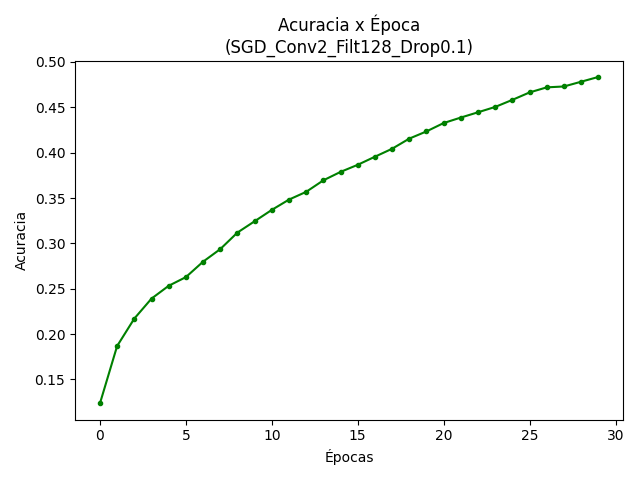
\includegraphics[width=\linewidth]{../../assets/cnn/SGD_Conv2_Filt128_Drop0.1_train_acuracia_plot.png}
        \caption*{SGD -- Acurácia de treino}
    \end{minipage}\hfill
    \begin{minipage}{0.48\textwidth}
        \centering
        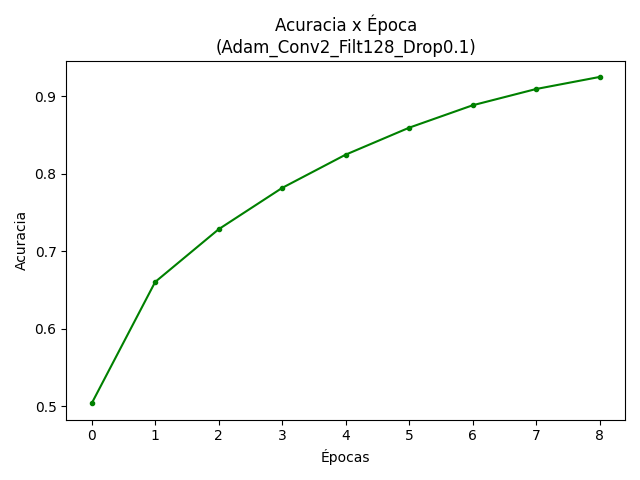
\includegraphics[width=\linewidth]{../../assets/cnn/Adam_Conv2_Filt128_Drop0.1_train_acuracia_plot.png}
        \caption*{Adam -- Acurácia de treino}
    \end{minipage}
\end{figure}

\begin{figure}[H]
    \centering
    \begin{minipage}{0.48\textwidth}
        \centering
        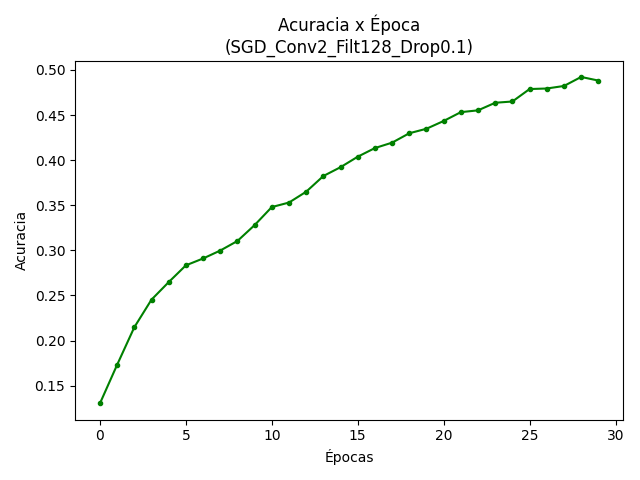
\includegraphics[width=\linewidth]{../../assets/cnn/SGD_Conv2_Filt128_Drop0.1_val_acuracia_plot.png}
        \caption*{SGD -- Acurácia de validação}
    \end{minipage}\hfill
    \begin{minipage}{0.48\textwidth}
        \centering
        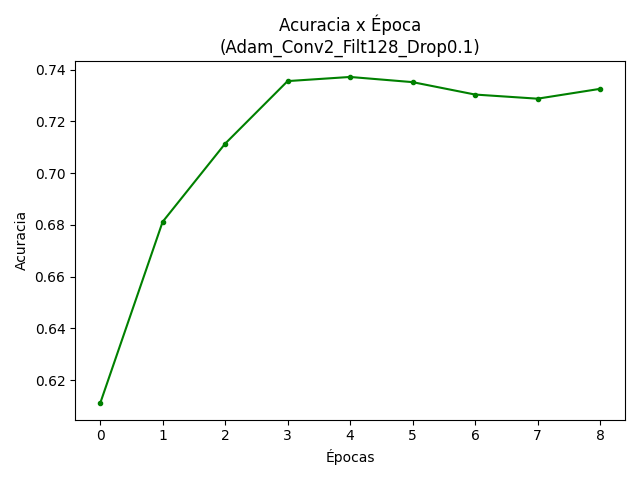
\includegraphics[width=\linewidth]{../../assets/cnn/Adam_Conv2_Filt128_Drop0.1_val_acuracia_plot.png}
        \caption*{Adam -- Acurácia de validação}
    \end{minipage}
\end{figure}

\begin{figure}[H]
    \centering
    \begin{minipage}{0.48\textwidth}
        \centering
        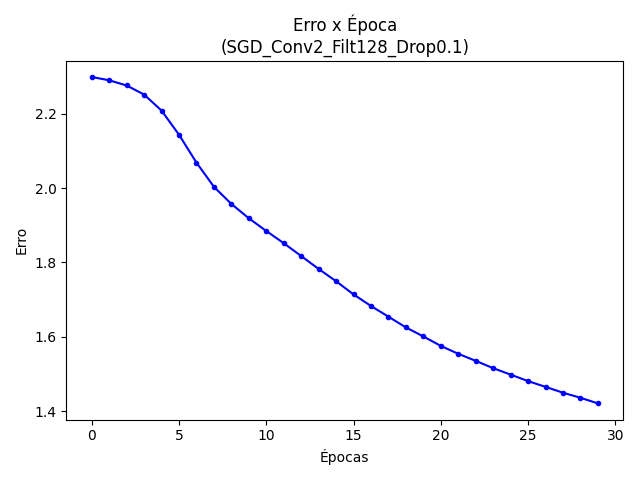
\includegraphics[width=\linewidth]{../../assets/cnn/SGD_Conv2_Filt128_Drop0.1_train_erro_plot.png}
        \caption*{SGD -- Erro de treino}
    \end{minipage}\hfill
    \begin{minipage}{0.48\textwidth}
        \centering
        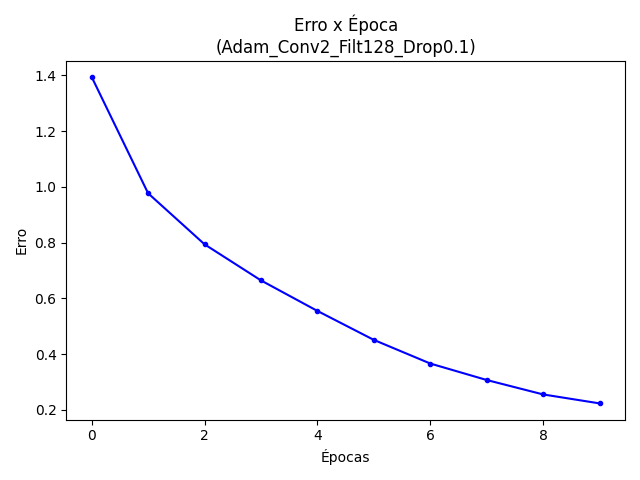
\includegraphics[width=\linewidth]{../../assets/cnn/Adam_Conv2_Filt128_Drop0.1_train_erro_plot.png}
        \caption*{Adam -- Erro de treino}
    \end{minipage}
\end{figure}

\begin{figure}[H]
    \centering
    \begin{minipage}{0.48\textwidth}
        \centering
        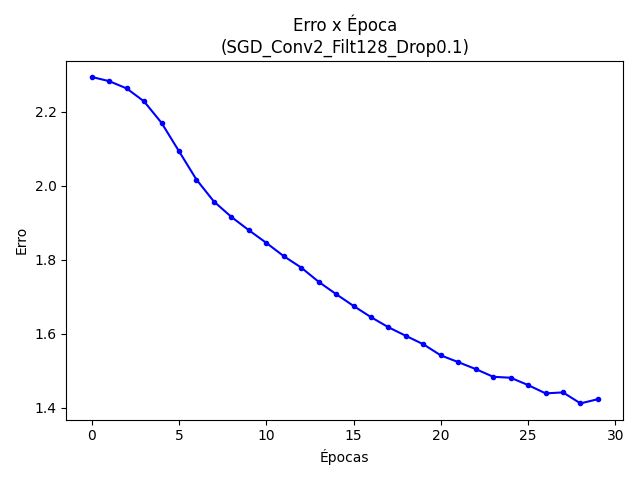
\includegraphics[width=\linewidth]{../../assets/cnn/SGD_Conv2_Filt128_Drop0.1_val_erro_plot.png}
        \caption*{SGD -- Erro de validação}
    \end{minipage}\hfill
    \begin{minipage}{0.48\textwidth}
        \centering
        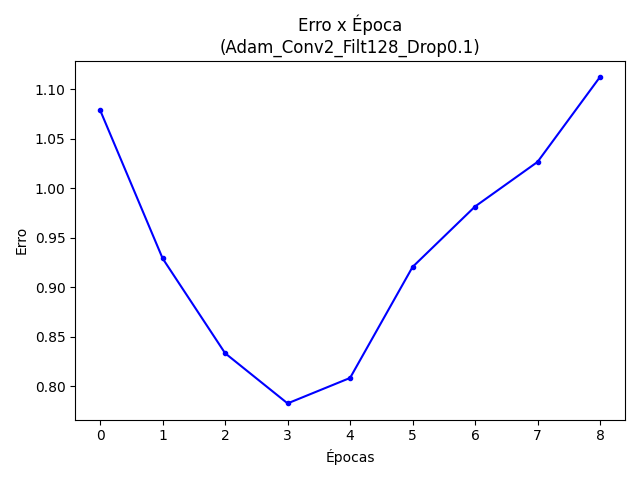
\includegraphics[width=\linewidth]{../../assets/cnn/Adam_Conv2_Filt128_Drop0.1_val_erro_plot.png}
        \caption*{Adam -- Erro de validação}
    \end{minipage}
\end{figure}

\subsection{Impacto do Número de Camadas Convolucionais}

Para o SGD, o desempenho piora monotonicamente com o aumento do número de camadas: 2 camadas resultam em acurácia média de $\approx$45\%, 3 camadas de $\approx$33\% e 4 camadas de $\approx$16\%. Isso indica que, sem uma taxa de aprendizado adaptativa, adicionar profundidade dificulta a otimização -- possivelmente por problemas de gradiente vanescente agravados pelo MaxPooling repetido que reduz o mapa espacial a $2\times2$ com 4 camadas.

Para o Adam, o padrão é diferente: 3 e 4 camadas convolucionais superam as arquiteturas com 2 camadas. A melhor acurácia geral (\textbf{76,46\%}) foi obtida com 4 camadas convolucionais, 128 filtros e $p=0{,}1$. Isso sugere que, com o otimizador adequado, maior profundidade extrai representações mais ricas e hierárquicas das imagens CIFAR-10.

\begin{figure}[H]
    \centering
    \begin{minipage}{0.32\textwidth}
        \centering
        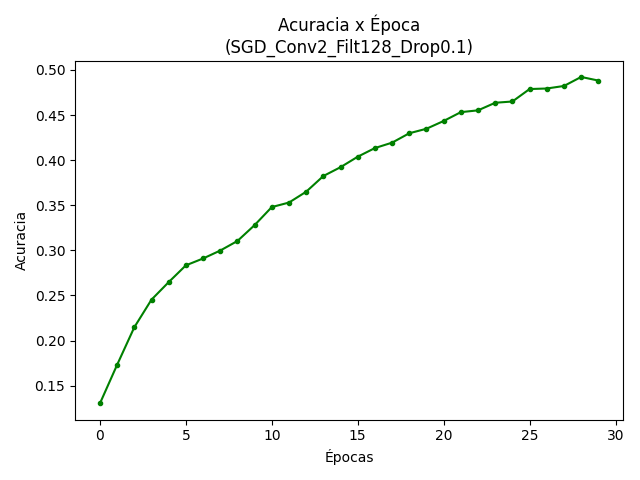
\includegraphics[width=\linewidth]{../../assets/cnn/SGD_Conv2_Filt128_Drop0.1_val_acuracia_plot.png}
        \caption*{SGD -- Conv2 (validação)}
    \end{minipage}\hfill
    \begin{minipage}{0.32\textwidth}
        \centering
        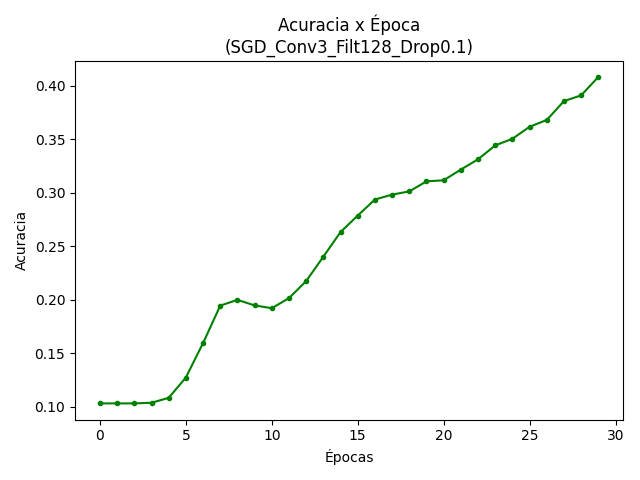
\includegraphics[width=\linewidth]{../../assets/cnn/SGD_Conv3_Filt128_Drop0.1_val_acuracia_plot.png}
        \caption*{SGD -- Conv3 (validação)}
    \end{minipage}\hfill
    \begin{minipage}{0.32\textwidth}
        \centering
        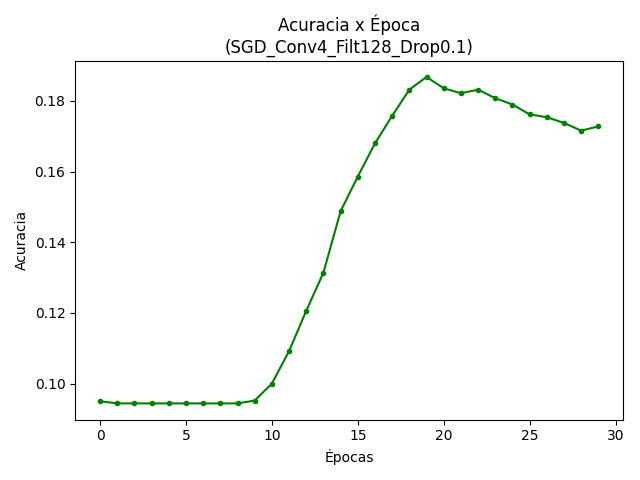
\includegraphics[width=\linewidth]{../../assets/cnn/SGD_Conv4_Filt128_Drop0.1_val_acuracia_plot.png}
        \caption*{SGD -- Conv4 (validação)}
    \end{minipage}
\end{figure}

\begin{figure}[H]
    \centering
    \begin{minipage}{0.32\textwidth}
        \centering
        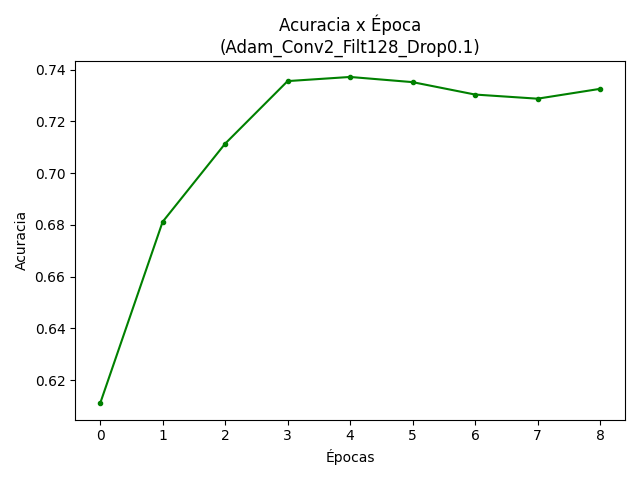
\includegraphics[width=\linewidth]{../../assets/cnn/Adam_Conv2_Filt128_Drop0.1_val_acuracia_plot.png}
        \caption*{Adam -- Conv2 (validação)}
    \end{minipage}\hfill
    \begin{minipage}{0.32\textwidth}
        \centering
        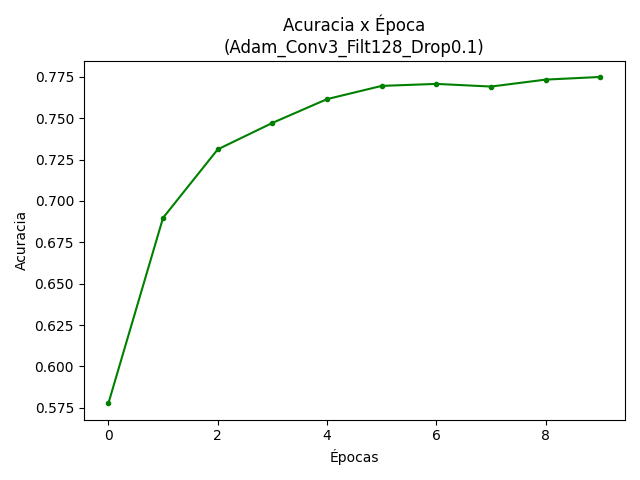
\includegraphics[width=\linewidth]{../../assets/cnn/Adam_Conv3_Filt128_Drop0.1_val_acuracia_plot.png}
        \caption*{Adam -- Conv3 (validação)}
    \end{minipage}\hfill
    \begin{minipage}{0.32\textwidth}
        \centering
        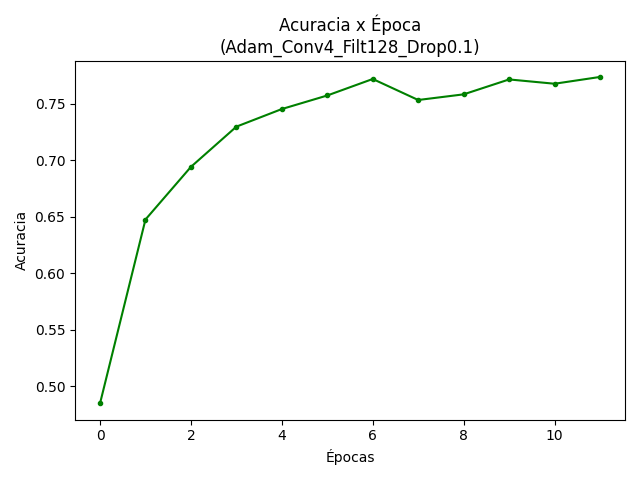
\includegraphics[width=\linewidth]{../../assets/cnn/Adam_Conv4_Filt128_Drop0.1_val_acuracia_plot.png}
        \caption*{Adam -- Conv4 (validação)}
    \end{minipage}
\end{figure}

\subsection{Impacto do Número de Filtros}

Em todas as configurações, aumentar o número de filtros melhora o desempenho. Para o Adam com 3 camadas convolucionais, a acurácia média sobe de $\approx$73\% com 32 filtros para $\approx$76\% com 128 filtros. Filtros adicionais permitem ao extrator de características capturar mais padrões visuais distintos por camada, o que é especialmente relevante para um dataset com 10 classes visualmente variadas.

\begin{figure}[H]
    \centering
    \begin{minipage}{0.32\textwidth}
        \centering
        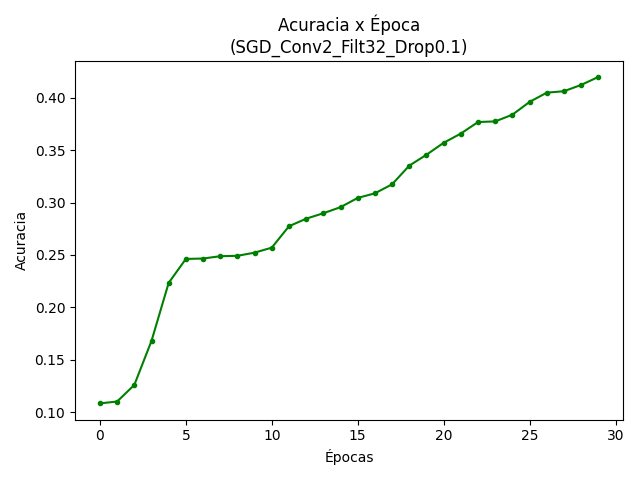
\includegraphics[width=\linewidth]{../../assets/cnn/SGD_Conv2_Filt32_Drop0.1_val_acuracia_plot.png}
        \caption*{SGD -- 32 filtros}
    \end{minipage}\hfill
    \begin{minipage}{0.32\textwidth}
        \centering
        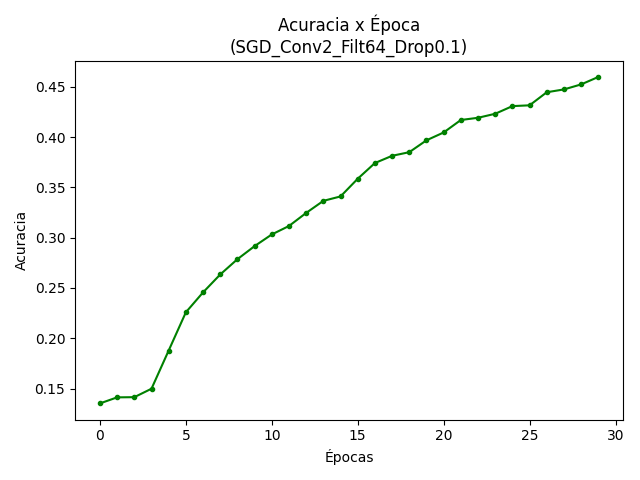
\includegraphics[width=\linewidth]{../../assets/cnn/SGD_Conv2_Filt64_Drop0.1_val_acuracia_plot.png}
        \caption*{SGD -- 64 filtros}
    \end{minipage}\hfill
    \begin{minipage}{0.32\textwidth}
        \centering
        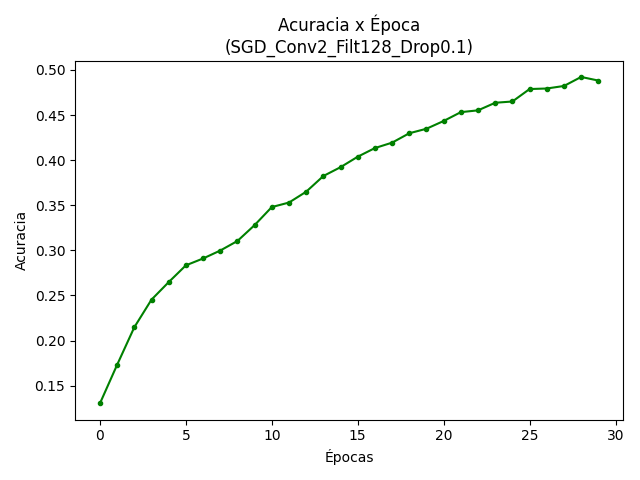
\includegraphics[width=\linewidth]{../../assets/cnn/SGD_Conv2_Filt128_Drop0.1_val_acuracia_plot.png}
        \caption*{SGD -- 128 filtros}
    \end{minipage}
\end{figure}

\begin{figure}[H]
    \centering
    \begin{minipage}{0.32\textwidth}
        \centering
        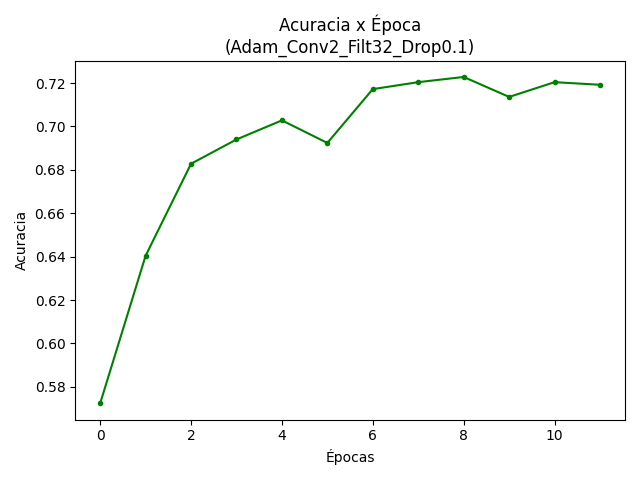
\includegraphics[width=\linewidth]{../../assets/cnn/Adam_Conv2_Filt32_Drop0.1_val_acuracia_plot.png}
        \caption*{Adam -- 32 filtros}
    \end{minipage}\hfill
    \begin{minipage}{0.32\textwidth}
        \centering
        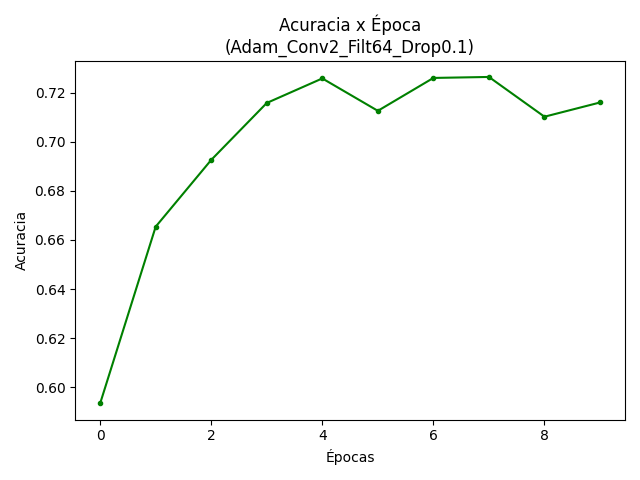
\includegraphics[width=\linewidth]{../../assets/cnn/Adam_Conv2_Filt64_Drop0.1_val_acuracia_plot.png}
        \caption*{Adam -- 64 filtros}
    \end{minipage}\hfill
    \begin{minipage}{0.32\textwidth}
        \centering
        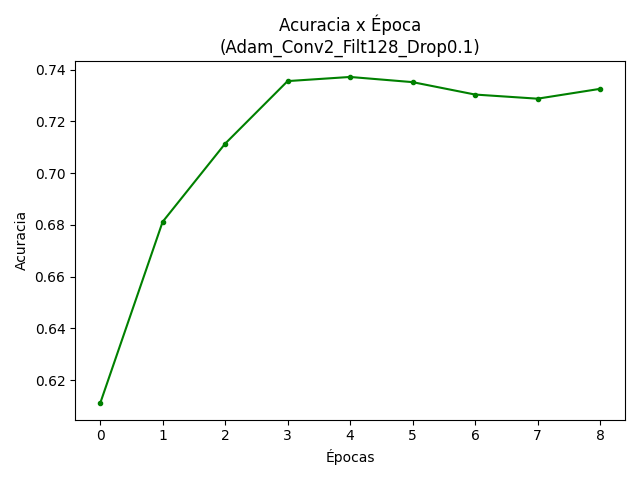
\includegraphics[width=\linewidth]{../../assets/cnn/Adam_Conv2_Filt128_Drop0.1_val_acuracia_plot.png}
        \caption*{Adam -- 128 filtros}
    \end{minipage}
\end{figure}

\subsection{Impacto do Dropout}

O impacto do dropout nas camadas FC foi sutil, porém observável. A tabela~\ref{tab:dropout} resume as médias por taxa de dropout separadas por otimizador.

\begin{table}[H]
\centering
\caption{Impacto do Dropout -- média de acurácia e loss no teste}
\label{tab:dropout}
\begin{tabular}{llll}
\toprule
\textbf{Otimizador} & \textbf{Dropout} & \textbf{Acc ($\mu$)} & \textbf{Loss ($\mu$)} \\
\midrule
SGD  & 0.1 & 0.3284 & 1.8639 \\
SGD  & 0.3 & 0.2974 & 1.9399 \\
Adam & 0.1 & 0.7309 & 0.9290 \\
Adam & 0.3 & 0.7316 & 0.8743 \\
\bottomrule
\end{tabular}
\end{table}

Para o SGD, o dropout $p=0{,}3$ prejudica levemente os resultados, possivelmente porque a rede já converge mal e o dropout adiciona mais variância ao gradiente. Para o Adam, os resultados são praticamente equivalentes entre $p=0{,}1$ e $p=0{,}3$, com uma leve vantagem de loss para $p=0{,}3$ (indicando menor sobreajuste) mas acurácia muito próxima. Isso sugere que, para esta arquitetura, o dropout nas camadas FC tem efeito marginal como regularizador, e que o principal fator diferenciador entre os modelos é o otimizador e a profundidade da rede.

\begin{figure}[H]
    \centering
    \begin{minipage}{0.48\textwidth}
        \centering
        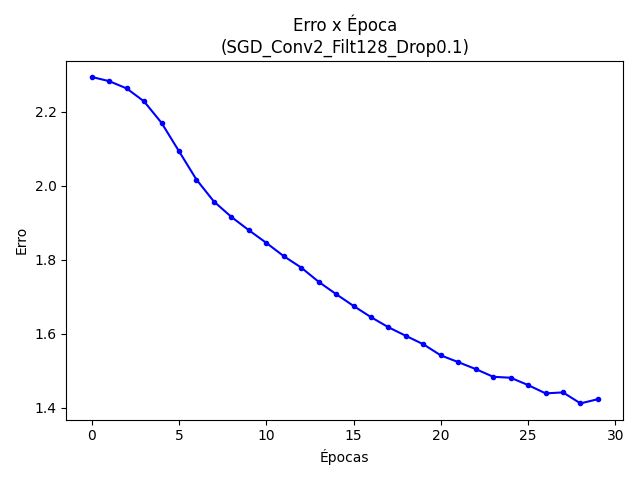
\includegraphics[width=\linewidth]{../../assets/cnn/SGD_Conv2_Filt128_Drop0.1_val_erro_plot.png}
        \caption*{SGD -- Dropout $p=0{,}1$ (validação)}
    \end{minipage}\hfill
    \begin{minipage}{0.48\textwidth}
        \centering
        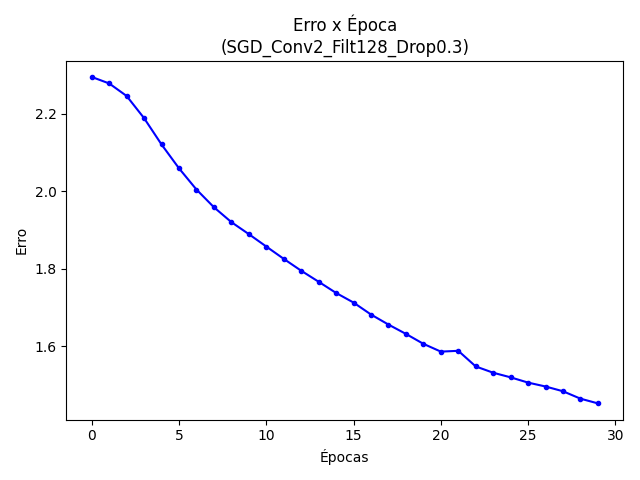
\includegraphics[width=\linewidth]{../../assets/cnn/SGD_Conv2_Filt128_Drop0.3_val_erro_plot.png}
        \caption*{SGD -- Dropout $p=0{,}3$ (validação)}
    \end{minipage}
\end{figure}

\begin{figure}[H]
    \centering
    \begin{minipage}{0.48\textwidth}
        \centering
        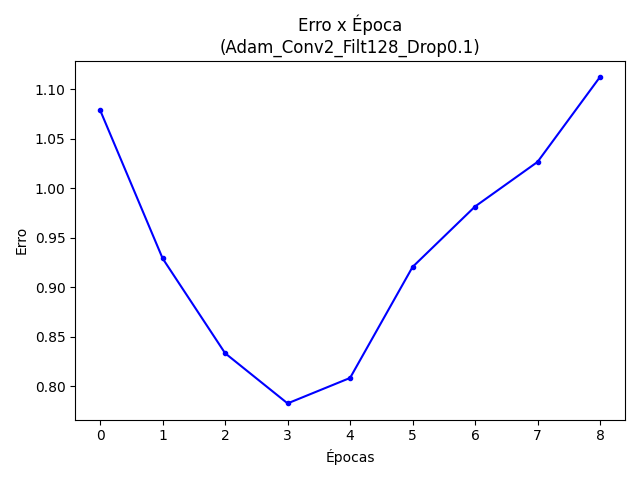
\includegraphics[width=\linewidth]{../../assets/cnn/Adam_Conv2_Filt128_Drop0.1_val_erro_plot.png}
        \caption*{Adam -- Dropout $p=0{,}1$ (validação)}
    \end{minipage}\hfill
    \begin{minipage}{0.48\textwidth}
        \centering
        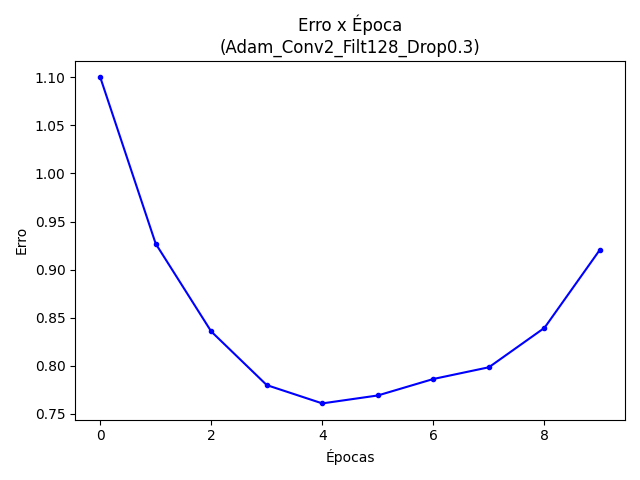
\includegraphics[width=\linewidth]{../../assets/cnn/Adam_Conv2_Filt128_Drop0.3_val_erro_plot.png}
        \caption*{Adam -- Dropout $p=0{,}3$ (validação)}
    \end{minipage}
\end{figure}

\subsection{Melhor Configuração}

\begin{table}[H]
\centering
\caption{Melhor configuração por otimizador (maior acurácia no teste)}
\label{tab:best}
\begin{tabular}{llllll}
\toprule
\textbf{Otim.} & \textbf{Conv} & \textbf{Filtros} & \textbf{Dropout} & \textbf{Loss} & \textbf{Acc} \\
\midrule
SGD  & 2 & 128 & 0.1 & 1.3779 & 0.5005 \\
Adam & 4 & 128 & 0.1 & 0.8780 & \textbf{0.7646} \\
\bottomrule
\end{tabular}
\end{table}

O melhor modelo geral foi \texttt{Adam\_Conv4\_Filt128\_Drop0.1}, com acurácia de \textbf{76,46\%} no teste, atingindo \textit{early stopping} na época 12. Para o SGD, o melhor resultado foi \texttt{SGD\_Conv2\_Filt128\_Drop0.1} com 50,05\% -- menos de 27 pontos percentuais abaixo do melhor Adam, o que é uma diferença expressiva.

\section{Conclusão}

Os experimentos com CNNs no CIFAR-10 revelam padrões distintos dos observados na MLP da atividade anterior. O otimizador Adam mostrou-se indispensável para a convergência das redes convolucionais neste contexto, enquanto o SGD falhou sistematicamente, especialmente em arquiteturas mais profundas.

O aumento de filtros e de camadas convolucionais beneficia o Adam de forma consistente, corroborando a intuição de que redes mais profundas extraem representações hierárquicas mais ricas. O dropout nas camadas FC, por sua vez, apresentou impacto marginal sobre a acurácia final, sendo o otimizador e a profundidade os fatores determinantes.

Respondendo às questões da atividade:

\textbf{Impacto do número de camadas e filtros:} Mais camadas e mais filtros melhoram a acurácia quando combinados com Adam. Com SGD, camadas adicionais prejudicam a convergência.

\textbf{Dropout e overfitting:} O dropout teve efeito limitado nesta configuração. A maior ameaça ao overfitting observada foram os modelos Adam com poucas épocas de treino, que ainda assim generalizaram razoavelmente bem.

\textbf{Generalização no conjunto de teste:} O melhor modelo (Adam, 4 convoluções, 128 filtros) atingiu 76,46\% de acurácia no teste, valor competitivo para uma CNN simples sem \textit{data augmentation} no CIFAR-10.

\end{document}
